\subsection{Lab12: Transmisor FM Estereo}

%*********************
\begin{frame}{}

\pgfdeclareimage[width=\paperwidth,height=\paperheight]{bg}{imagenes/fondo_lab}
\setbeamertemplate{background}{\pgfuseimage{bg}}

\bfseries{\textrm{\LARGE Lab12\\ \Large Transmisor FM Estereofónico}}
\raggedright
\end{frame}
%*********************


\begin{frame}{Transmisión FM stereo}

\pgfdeclareimage[width=\paperwidth,height=\paperheight]{bg}{imagenes/fondo3}
\setbeamertemplate{background}{\pgfuseimage{bg}}

La transmisión FM stereo es la emisión en frecuencia modulada por dos canales. Para emitir en stereo no se emite directamente la señal R (Right ó Derecha) y la señal L (Left ó Izquierda) sino que se emiten las señales L-R por un canal y L+R por el otro. Esto se realiza con el fin de dar cualidades y calidades de sonido stero a la transmisión por frecuencia modulada.

\end{frame}
%---------------------------------

\begin{frame}{Transmisión FM stereo}
    
\begin{figure}[H]
\centering
\vspace{-3mm}
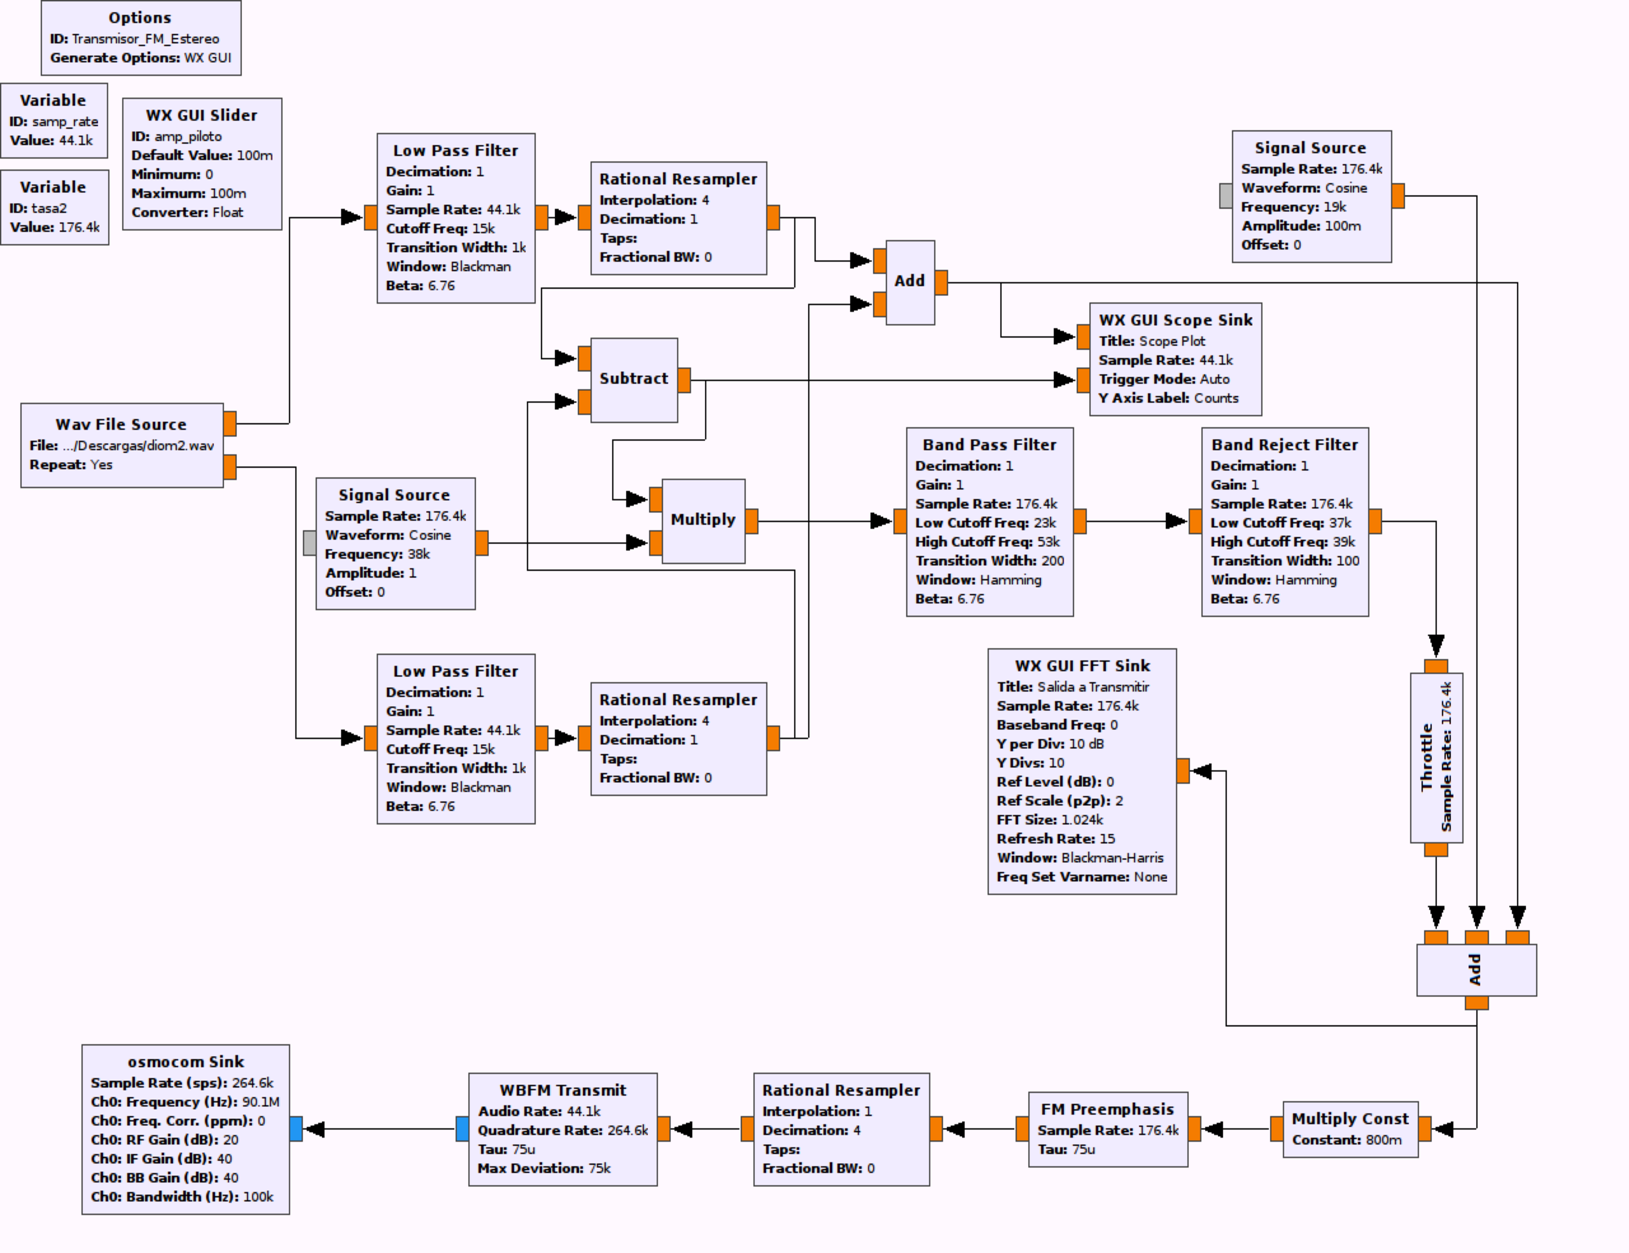
\includegraphics[width=.8\textwidth]{parte3/lab12/pdf/lab12_1.pdf}
\end{figure}
    
\end{frame}
%---------------------------------

\begin{frame}{Transmisión FM stereo}

\begin{figure}[H]
\centering
\vspace{-3mm}
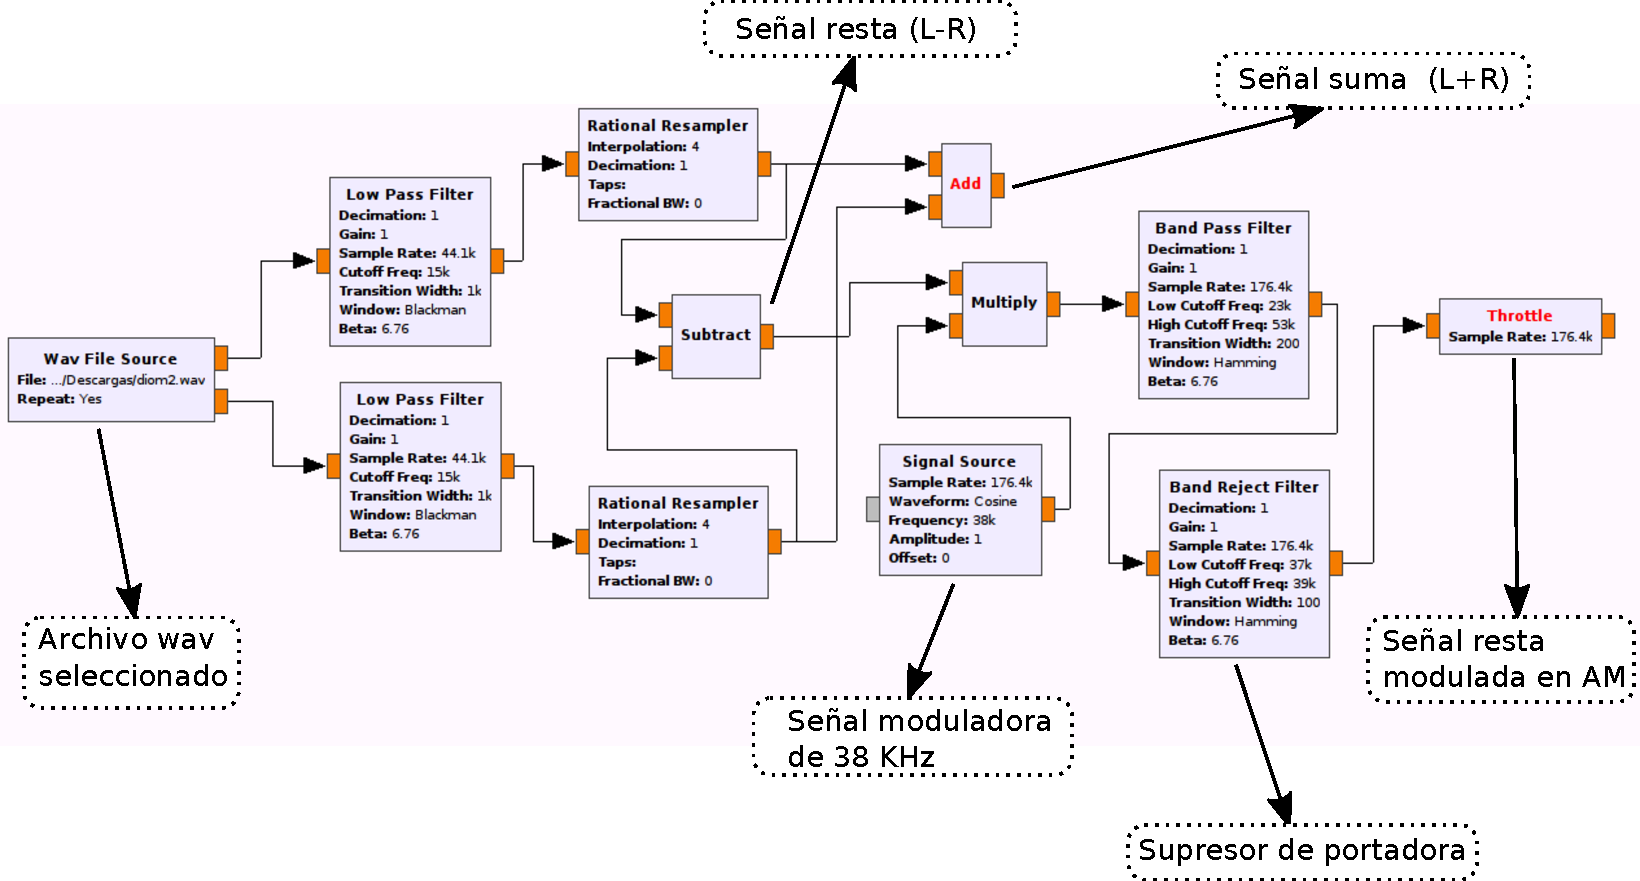
\includegraphics[width=\textwidth]{parte3/lab12/pdf/lab12_2.pdf}
\end{figure}
    
\end{frame}
%---------------------------------

\begin{frame}{Transmisión FM stereo}

\begin{figure}[H]
\centering
\vspace{-3mm}
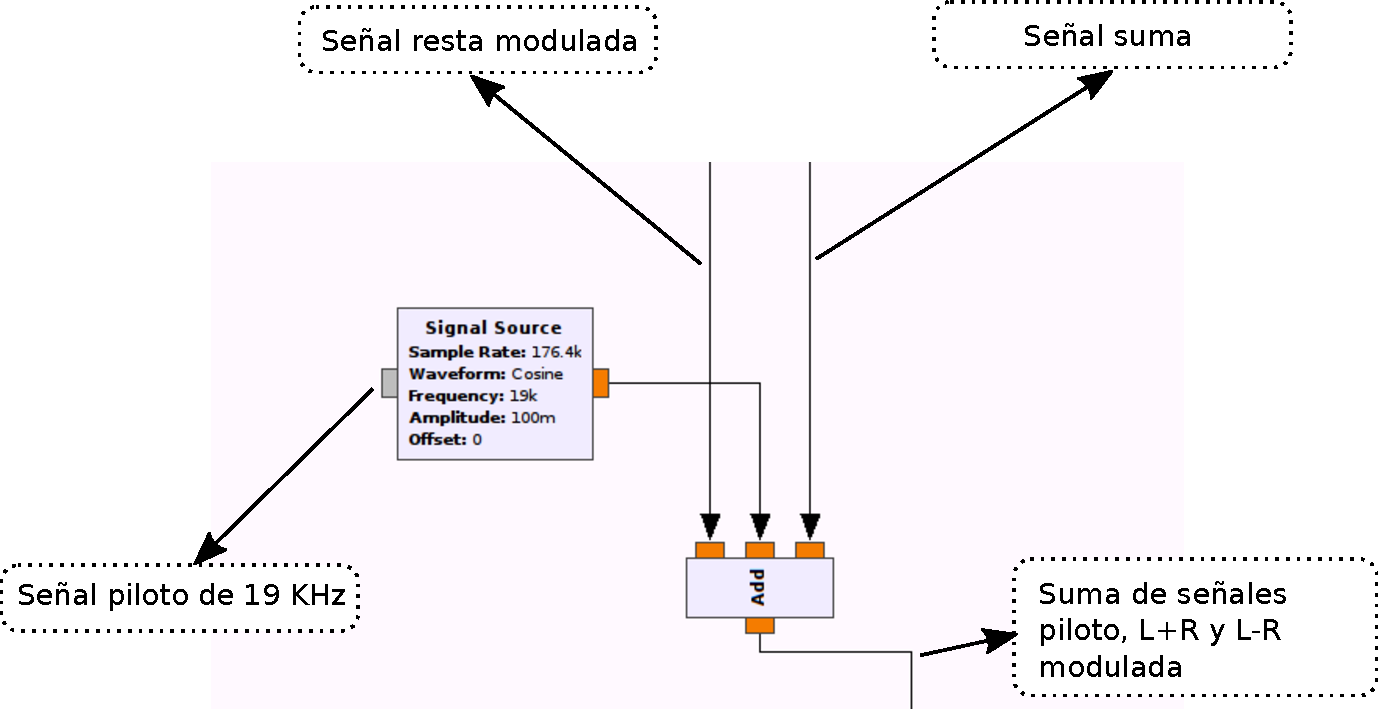
\includegraphics[width=\textwidth]{parte3/lab12/pdf/lab12_3.pdf}
\end{figure}
    
\end{frame}
%---------------------------------

\begin{frame}{Señal piloto de 19 KHz}

 El piloto estéreo es un tono de 19kHz que tiene la misma fase que la portadora de la Señal Resta (que hemos eliminado previamente), y una amplitud de (normalmente) el 10\% de la amplitud total de la señal, en caso de no detectarse el piloto es conveniente aumentar la amplitud del mismo hasta ser detectada por el receptor.
El piloto estéreo tiene tres funciones principales:

\begin{itemize}
    \item {Informa al receptor de que la emisión es estéreo}
    \item{Permite regenerar la subportadora de la Señal Resta a 38kHz que no hemos emitido gracias a modular en DSBSC.}
    \item{Permite regenerar la subportadora del RDS a 57kHz que no hemos emitido gracias a modular en DSBSC.}
\end{itemize}
    
\end{frame}
%---------------------------------

\begin{frame}{Transmisión FM stereo}

\begin{figure}[H]
\centering
\vspace{-3mm}
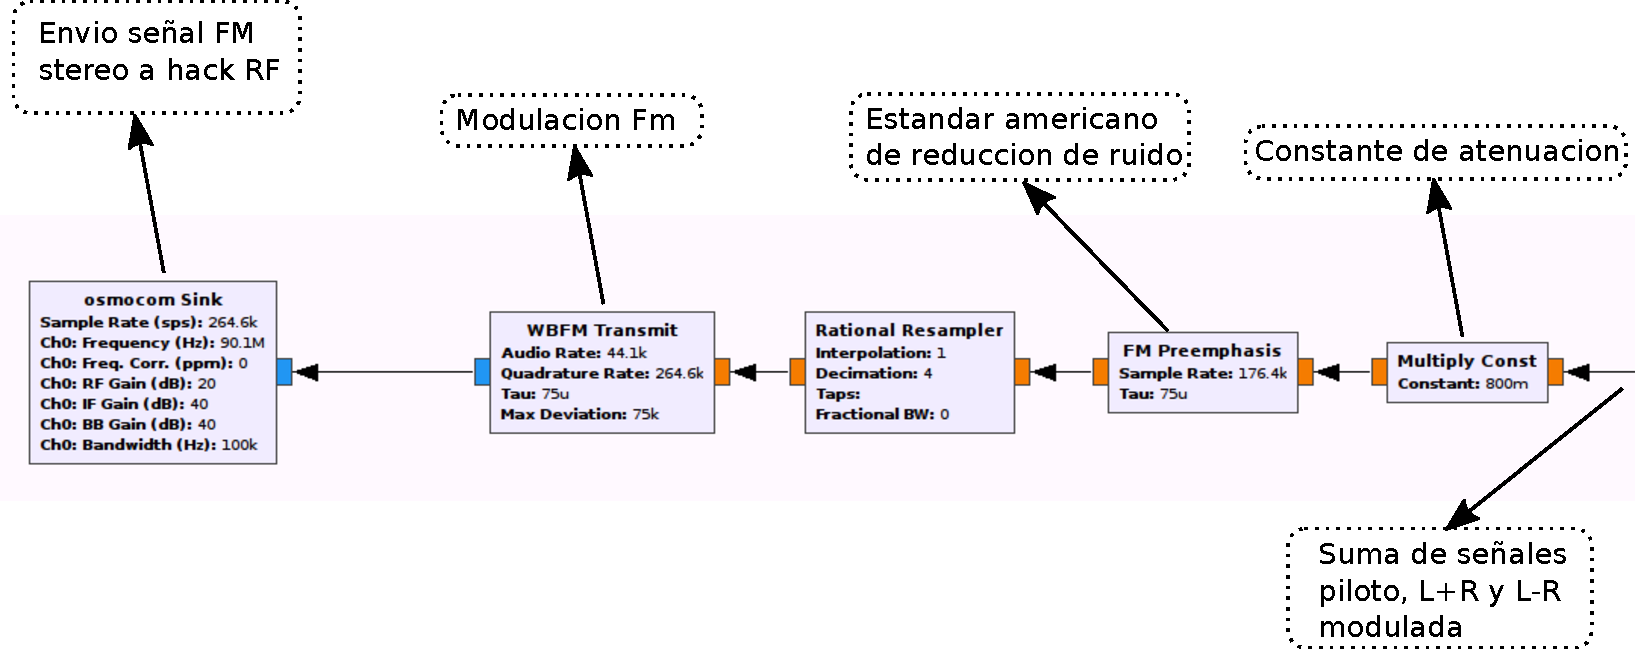
\includegraphics[width=\textwidth]{parte3/lab12/pdf/lab12_4.pdf}
\end{figure}
    
\end{frame}
%---------------------------------

\begin{frame}{Transmisión FM stereo}

\begin{figure}[H]
\centering
\vspace{-3mm}
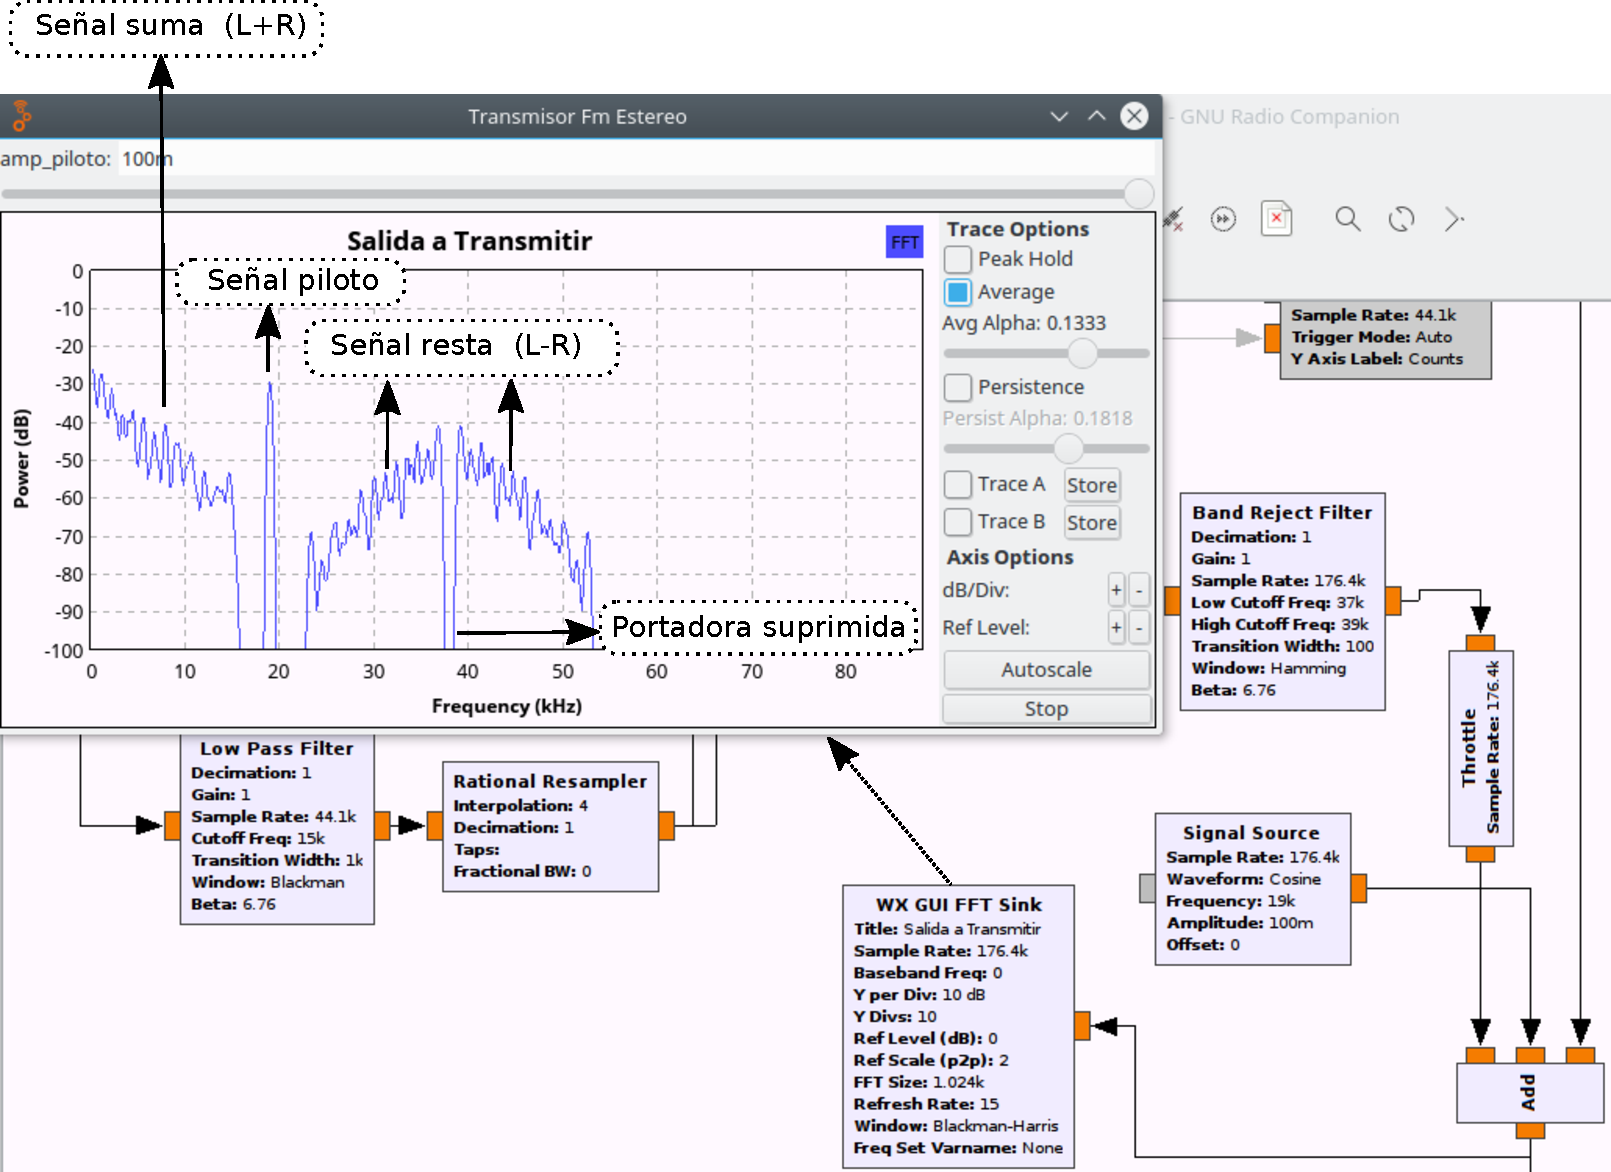
\includegraphics[width=.9\textwidth]{parte3/lab12/pdf/lab12_5.pdf}
\end{figure}
    
\end{frame}
%---------------------------------